\chapter{Designing Classes}

\section{Exercises}

\begin{exercise}
Define a class named \java{Lens} that represents a camera lens by its focal length (distance from lens to sensor) and aperture (diameter of lens opening), both measured in millimeters. These will be stored in two \java{private double} instance variables. Implement the following:

\begin{enumerate}
\item A default constructor that sets both attributes to 1.0.

\item A two-argument constructor that sets the attributes as specified by the caller (setting a value to 1.0 if the argument is less than zero).

\item Write getters and setters for both attributes. Again, the mutator sets a value to 1.0 if given an argument less than zero by the caller.

\item Write an instance method named \java{calcFStop} that returns the lens's f-stop value by dividing the focal length by the aperture.

\item Provide a \java{toString} method to display the focal length and aperture, properly labeled, with one digit to the right of the decimal point.

\item Implement an \java{equals} instance method that takes another \java{Lens} object as its parameter and returns \java{true} if the two lenses have the same focal length and aperture, \java{false} otherwise.

\item The \java{main} program will ask the user for two sets of focal length and aperture and will create corresponding \java{Lens} object. It will then display the first \java{Lens}'s attributes and f-stop. If the second \java{Lens} is not equal to the first one, it will also display the second \java{Lens}'s attributes and f-stop; otherwise, it will output a message that the two lenses are the same.
\end{enumerate}

Here is some sample output from running the program twice:

\begin{stdout}
Enter focal length of first lens in mm: 3.5
Enter aperture of first lens in mm: 2

Enter focal length of second lens in mm: 4.3
Enter aperture of second lens in mm: 3

First lens: focal length: 3.5mm, aperture: 2.0mm; f-stop 1.8
Second lens: focal length: 4.3mm, aperture: 3.0mm; f-stop 1.4

// ===================

Enter focal length of first lens in mm: 3.5
Enter aperture of first lens in mm: 2

Enter focal length of second lens in mm: 3.5
Enter aperture of second lens in mm: 2

First lens: focal length: 3.5mm, aperture: 2.0mm; f-stop 1.8
The second lens is the same as the first one.
\end{stdout}

\end{exercise}

\begin{exercise}

In an {\em n}-sided regular polygon, all sides have the same length and all angles have the same degree (i.e., the polygon is both equilateral and equiangular). Design a class named \java{RegularPolygon} that contains:
\begin{itemize}
    \item A private \java{int} data field named \java{nSides} that defines the number of sides in the polygon with default value 3.
    \item A private \java{double} data field named \java{sideLength} that stores the length of the side, with default value 1.0
    \item A private \java{double} data field named \java{x} that defines the {\em x}-coordinate of the polygon's center with default value 0.0
    \item A private \java{double} data field named \java{y} that defines the {\em y}-coordinate of the polygon's center with default value 0.0
    \item A no-argument constructor that creates a regular polygon with default values
    \item A constructor that creates a regular polygon with the specified number of sides and length of side, centered at (0, 0)
    \item A constructor that creates a regular polygon with the specified number of sides, length of side, and {\em x-}and {\em y-} coordinates
    \item The accessor and mutator methods (getters and setters) for all data fields
    \item The method \java{getPerimeter} that returns the perimeter of the polygon
    \item The method \java{getArea} that returns the area of the polygon. The formula for computing the area of a regular polygon is:
    
    \begin{equation*}
    {{n \times s^2} \over {4 \times tan({\pi \over n})}}
    \end{equation*}
    \item An \java{equals} instance method that takes another \java{RegularPolygon} object as its parameter and returns \java{true} if the two polygons have the same number of sides and side length, \java{false} otherwise.
    
\end{itemize}

Draw the UML diagram for the class, then implement the class.

Write a test program named {\em PolygonTest.java}. The test program will create three \java{RegularPolygon} objects, created using:
\begin{itemize}
    \item The no-argument constructor
    \item \java{RegularPolygon(6, 4.0)}
    \item \java{RegularPolygon(10, 4, 5.6, 7.8)}
\end{itemize}

For each object, display its perimeter and area, properly labeled. Format the values to three decimal places.

Put the \java{RegularPolygon} class in the {\em PolygonTest.java} file rather than creating a separate file for the class. 
\end{exercise}

\begin{exercise}
This program will implement a class to represent the data in a bank account; you will also write a class with a \java{main} method to test this class.

The \java{Account} class has two \java{private} instance variables:  \java{acctNumber}, which is an \java{int}, and  \java{balance}, which is a \java{double}.

Implement the following methods:

\begin{itemize}
\item A two-argument constructor that specifies the account number and starting balance for the account. (In this program, you won't write a no-argument constructor.) If the starting balance is less than zero, leave it unchanged---its value will be zero, because that is the default value for a \java{double} instance variable.

\item A getter method for the account number. It will be called \java{getAcctNumber}. Do {\em not} write a setter method---once you establish an account number in the constructor, it should never be changed.

\item Both a getter and setter method for the balance. If the setter is given a balance less than zero, leave the current account balance unchanged.

\item A \java{toString} method that returns a \java{String} with the account number and balance, properly labeled. You must display the balance with a currency symbol and exactly two digits to the right of the decimal point.

\item A \java{void} method named \java{deposit} that accepts a \java{double} amount as its single parameter. If the amount is negative, leave the balance untouched. Otherwise, add the amount to the balance.

\item A \java{void} method named \java{withdraw} that accepts a \java{double} amount as its single parameter. If the amount is negative or greater than the balance, leave the balance untouched. Otherwise, subtract the amount from the balance.

\end{itemize}

None of the preceding methods prints anything. If someone gives bad input to \java{deposit} or \java{withdraw}, the caller (in this instance, \java{main}) is responsible for doing appropriate error handling. However, because you can't count on the users to handle errors correctly all the time, it's up to you to make sure that the methods always do something reasonable---in this case, leaving the balance alone rather than changing it to an invalid value.

Draw a UML diagram for the class and implement it.

Finally, write a class named \java{TestAccount} with a \java{main} method that does the following:

\begin{enumerate}
\item Create an \java{Account} variable for account number 1047217, with an initial balance of \$1732.00. 

\item Display the account variable you created in the previous step. {\em Hint}: use \java{toString}.

\item Deposit \$450.25 to the account and display it.

\item Withdraw \$301.75 from the account and display it.

\item Deposit -\$22.33 to the account and display it. The balance should not be changed.

\item Withdraw -\$44.55 from the account and display it. The balance should not be changed.

\item Withdraw \$2000.00 from the account and display it. The balance should not be changed.
\end{enumerate}

Here is what the output might look like:

\begin{stdout}
Account 1047217 has balance $1732.00
Deposit $450.25: Account 1047217 has balance $2182.25
Withdraw $301.75: Account 1047217 has balance $1880.50
Deposit -$22.33: Account 1047217 has balance $1880.50
Withdraw -$44.55: Account 1047217 has balance $1880.50
Withdraw $2000: Account 1047217 has balance $1880.50
\end{stdout}
\end{exercise}

\begin{exercise}
This program will implement two classes, and you will draw a UML diagram for first of these classes.

First, implement a class named \java{InventoryItem} that contains these instance variables:

\begin{itemize}
    \item A private \java{String} data field named \java{itemName} that gives the name of the item. Its default value is \java{"TBD"}.
    \item A private \java{int} data field named \java{sku}. An SKU (stock keeping unit) is like an ID number for an item. Its default value is zero.
    \item A private \java{double} data field named \java{price} that stores the price for the item. The default value is 0.0.
    \item A private \java{int} data field named \java{quantity} that tells how many items are in stock. The default value is 0.
\end{itemize}

Implement the following methods, all of which must be \java{public}:

\begin{itemize}
    \item A no-argument constructor that creates an inventory item with default values.
    \item A three-argument constructor that creates an inventory item with the specified name, SKU, and price (in that order) with the default quantity.
    \item A four-argument constructor that creates an inventory item with the specified name, SKU, price, and quantity (in that order).
    \item The accessor and mutator methods (getters and setters) for all the instance fields.
    \item A method named \java{getTotalValue()} which returns, as a double, the item price times its quantity.
    \item A \java{toString()} method that returns a \java{String} with the item's name, SKU, price, and quantity, properly labeled. It must {\em not} include the total value; that is not an attribute of the object.
    \item A static method named \java{compare()} which takes as its arguments two \java{InventoryItem} objects. This method returns:
        \begin{itemize}
            \item -1 if the total value of the first item is less than the total value of the second item
            \item 0 if the total value of the first item equals the total value of the second item
            \item 1 if the total value of the first item is greater than the total value of the second item
        \end{itemize}
        
For example, if \java{item1} has a price of \$2.00 and a quantity of 9, and \java{item2} has a price of \$3.00 and a quantity of 5, \java{InventoryItem.compare(item1, item2)} would return 1 because the total value of \java{item1} (\$18.00) is greater than the total value of \java{item2} (\$15.00).
        
This method {\em must} call the \java{getTotalValue()} method.
    
\end{itemize}

Note: if the constructors and setters are given a negative price or quantity, they must convert it to a positive number. Hint - use \java{Math.abs()}.

Draw a UML diagram for this class. 

Next, implement the \java{TestInventory} class, which will contain your \java{main()} method and will do the following:

\begin{itemize}
    \item Create four \java{InventoryItem}s:
        \begin{itemize}
            \item \java{emptyItem}, using the no-argument constructor
            \item \java{staplers}, which has a name of "Stapler, Red", SKU of 91745, and price of \$7.89, using the three-argument constructor
            \item \java{pencils}, which has a name "Pencil, \#2", SKU of 73105, price of \$0.35, and quantity 210
            \item \java{notebooks}, which has a name "Notebook, Spiral", SKU of 68332, price of \$2.57, and quantity 38
        \end{itemize}
    
    \item Display each of the items (using the \java{display()} method) and its total value.
    \item Compare \java{pencils} to \java{notebooks} and prints out which one has greater total value. You must call the \java{compare()} method as part of this step . Output must use the inventory item's \java{itemName} property.
\end{itemize}

Here is what output from the program might look like. Your output does not have to look exactly like this, but it must reflect the same information.

\begin{stdout}
TBD [SKU 0]: 0 at $0.00 each
Total value: $0.00

Stapler, Red [SKU 91745]: 0 at $7.89 each
Total value: $0.00

Pencil, #2 [SKU 73105]: 210 at $0.35 each
Total value: $73.50

Notebook, Spiral [SKU 68332]: 38 at $2.57 each
Total value: $97.66

Notebook, Spiral has greater value than Pencil, #2
\end{stdout}
\end{exercise}

\begin{exercise}
One advantage of making instance variables \java{private} is that they allow you to hide the implementation details from users. You provide an API (application program interface---a set of methods for accessing the data), and users interact with the data through those methods. This frees you to change the underlying implementation at any time.

For example, consider a three-dimensional vector. You might be tempted to create a class with these instance variables \java{x}, \java{y}, and \java{z}, as in the UML diagram of Figure~\ref{fig.vec3d_a}:

\begin{figure}[!h]
\begin{center}
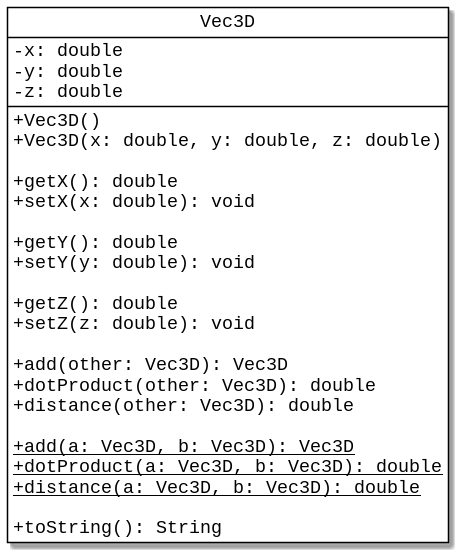
\includegraphics[scale=0.5]{figs/ch11/vec3d_a.png}
\caption{UML Diagram with three separate instance variables}
\label{fig.vec3d_a}
\end{center}
\end{figure}

The class has a no-argument constructor (which sets all the coordinates to zero) and a three-argument constructor to set the {\em x}, {\em y}, and {\em z} coordinates explicitly.

These are followed by the getters (accessors) and setters (mutators) for each of the dimensions. 

The class specifies an \java{add}, \java{dotProduct}, and \java{distance} instance methods that find the sum, dot product, and distance of the current vector and an ```other'' vector.

For the convenience of users, the class also specifies \java{static} versions of these methods (the convention in UML diagrams is to underline \java{static} elements) where you specify both vectors you want to manipulate.


But wait---you already have code for doing addition, dot product, and vector distance from Exercise~\ref{ex:vectors}. Because your instance variables are private, you can replace \java{x}, \java{y}, and \java{z} with a three-element array of \java{double} values, as in Figure~\ref{fig.vec3d_b}, and use the code that you wrote in that exercise.

\begin{figure}[!h]
\begin{center}
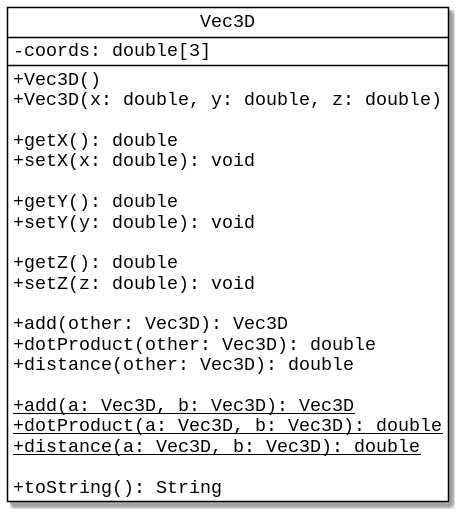
\includegraphics[scale=0.5]{figs/ch11/vec3d_b.png}
\caption{UML Diagram with array to hold coordinates}
\label{fig.vec3d_b}
\end{center}
\end{figure}

Notice that the \java{public} methods have not changed; users will never know that the vector is implemented as an array rather than three individual variables.

And that's your job for this exercise: implement the \java{Vec3D} class with a \java{private} array to hold the coordinates. Then, write a \java{main} method that will ask the user to enter two vectors and then display the sum, dot product, and distance between the vectors. To avoid repetitious code, you might want to write a \java{getVector} method that has a prompt and a \java{Scanner} as its parameters. This method will prompt the user for the three vector components and return a \java{Vec3D} object. 

\end{exercise}
